\documentclass[crop,tikz]{standalone}
\usetikzlibrary{backgrounds}
\colorlet{blue}{cyan}
\tikzset{
  inverted/.style = {
    color=white,
    background rectangle/.style={fill},
    show background rectangle
  }
}

\usepackage{pgfplots}
\tikzset{>=latex}
\usepgfplotslibrary{colormaps}

\begin{document}
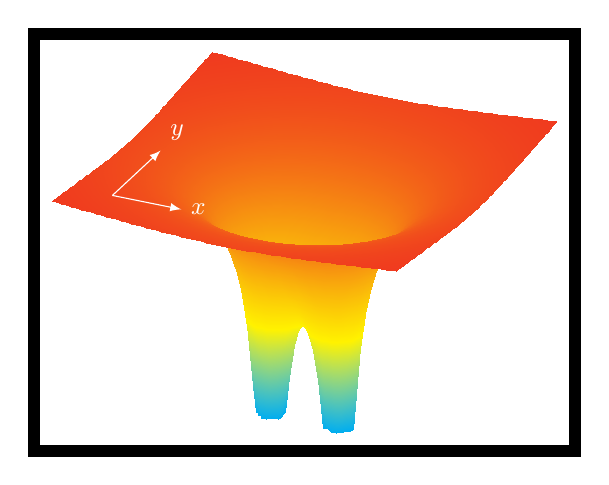
\begin{tikzpicture}[inverted,inverted]
  \begin{axis}[inverted,
    width=8cm,
    height=8cm,
    domain=-5:5,
    shader=interp,
    colormap/hot,
    point meta min=-3,
    point meta max=0,
    hide axis,
    zmin=-3, zmax=0,
    clip=false,
    declare function = { f(\x,\y) = -1/sqrt((\x+1)^2 + (\y)^2) - 1/sqrt((\x-1)^2 + (\y)^2); },
    ]
    \addplot3[
       restrict z to domain* = -3:0,
       surf,
       samples=70,
    ]{ f(x,y) };
    \node[white] at (axis cs: 3, 5, 0) { $\phi(\vec{r})$ };
    \coordinate (O) at (axis cs: -3, -5.5, 0); % origin
    \draw[->, white] (O) -- (axis cs: -1, -5.5, 0) node[right] { \small $x$ };
    \draw[->, white] (O) -- (axis cs: -3, -2.5, 0) node[above right] { \small $y$ };
  \end{axis}
\end{tikzpicture}
\end{document}
